\begin{frame}{Information Retrieval}
    
    \begin{figure} [H]
        \begin{center}
            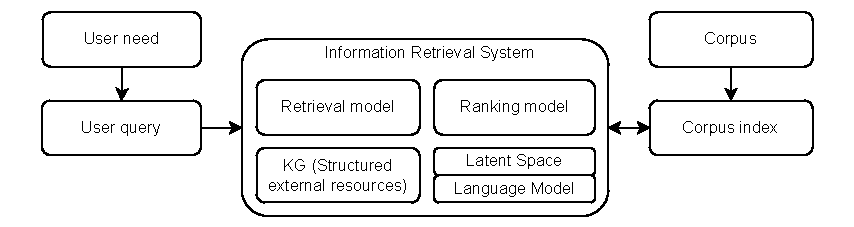
\includegraphics[scale=0.8]{images/ir-system-comps.pdf} 
            \caption{Information Retrieval System overview} 
        \end{center}
    \end{figure}

    \begin{center}
        Traditional approaches leverage statistics about the text corpus. Recent methods implement deep learning models.
    \end{center}
    
\end{frame}

\begin{frame}{BM25}

    \begin{itemize}
        \item The more structured the content is the better.
        \item Systems combines multiple methods balanced with parameters.
        \item Deep Learning methods requires relatively long texts.
    \end{itemize}
    
    BM25 (and its many variants) is:
    \begin{itemize}
        \item based on the Term Frequencies and Inverse Document Frequencies (TF-IDF)
        \item still widely used in practice
        \item computes many statistics offline
    \end{itemize}

    \begin{center}
        Traceparts search system is largely based on a BM25 implementation.
    \end{center}
    
\end{frame}

\begin{frame}{Traceparts search system}
    
    \begin{center}
        A text-based search engine.
    \end{center}
    
    \begin{figure} [H]
        \begin{center}
            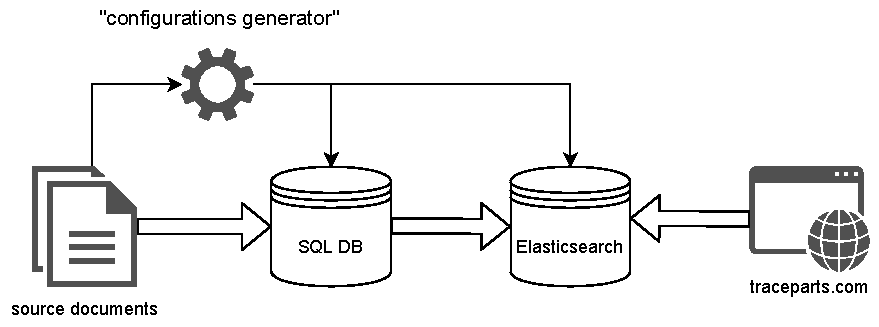
\includegraphics[scale=0.7]{images/tp_system.pdf} 
            \caption{Traceparts current system} 
        \end{center}
    \end{figure}

    \begin{center}
        Parts configurations are generated with their text content to be searchable.    
    \end{center}
    
\end{frame}

\begin{frame}{Traceparts search system challenges}
    
    Traceparts search challenges come from:
    \begin{itemize}
        \item Short multilingual texts
        \item Technical texts with many synonyms, acronyms, homonyms, and notations
        \item A large and heterogeneous corpus
        \item Multiple engineering domains coverage
        \item High recall but low precision
    \end{itemize}

\end{frame}